\documentclass[paper=letter, fontsize=12pt]{scrartcl}
\usepackage{amsmath, amssymb, latexsym}
\usepackage{anyfontsize}
\usepackage[utf8]{inputenc}
\usepackage[spanish]{babel}
\usepackage[utf8]{inputenc}
\usepackage{forest}
\usepackage{MnSymbol}
\usepackage{wasysym}
\usepackage{multicol}
\graphicspath{ {images/} }
\DeclareGraphicsExtensions{,.pdf,.png,.jpg,.gif}
\begin{document}
\parindent=0mm:
	\begin{center}
  Estructuras Discretas 2017-1\\
  Tarea 6\\
\end{center}

Alumno: Luis Alberto Martinez Monroy\\
N cuenta: 314212391\\ \\

{\Large{\bf 1.- Utilizando Tableaux (*)}}\\
{\bf a) Encuentra todos los modelos de la siguiente expresion logica}\\
\begin{center}
$\neg ((\neg p \vee \neg q) \rightarrow \neg (p \wedge r))$\\
$\equiv \neg (\neg(\neg p \vee \neg q) \vee \neg (p \wedge r))$\\
$\equiv \neg \neg(\neg p \vee \neg q) \wedge \neg \neg (p \wedge r)$\\
$\equiv (\neg p \vee \neg q) \wedge(p \wedge r))$\\
\begin{forest}

[$(\neg p \vee \neg q) \wedge (p \wedge r)$
	[$\neg p \vee \neg q$
		[$p\wedge r$
			[$p$
				[$r$
					[$\neg p$
						[cancelado]
					]
					[$\neg q$
						[modelo]
					]
				]
			]
		]
	]
]
\end{forest}
\end{center}
Los modelos para la expreción $\neg (\neg p \vee \neg q) \rightarrow \neg (p \wedge r)$ son:\\
modelo 1:\\
I (p)= 1\\
I (r)= 1\\
I (q)= 0\\
\newpage
{\bf b) Decidir si la siguiente fórmula es tautología}\\
\begin{center}
$(p\rightarrow \neg q \wedge r) \rightarrow (p\rightarrow p\rightarrow q\rightarrow r)$\\
$\equiv \neg(p\rightarrow \neg q \wedge r)\vee (p\rightarrow q \rightarrow r)$\\
$\equiv \neg (\neg p \vee (\neg q\wedge r))\vee (p\rightarrow \neg q \vee r)$\\
$\equiv \neg (\neg p \vee(\neg q \wedge r))\vee (\neg p \vee (\neg q \vee r))$\\
$\equiv (\neg \neg p \wedge \neg(\neg q \wedge r))\vee (\neg p \vee (\neg q \vee r))$\\
$\equiv (p\wedge(\neg \neg q \vee \neg r))\vee (\neg p \vee (\neg q \vee r))$\\
$\equiv (p\wedge (q \vee \neg r))\vee (\neg p \vee(\neg q \vee r))$\\
Ahora la negamos para que si es tautologia, el diagrama nos de una contradiccion.
$\neg ((\neg p\wedge (q\vee \neg r))\vee (\neg p \vee (\neg q \vee r)))$\\
$\equiv \neg(p\wedge (q\vee \neg r))\wedge \neg(\neg p \vee (\neg q \vee r))$\\
$\equiv (\neg p \vee \neg (q\vee \neg r))\wedge (\neg \neg p \wedge \neg(\neg q \vee r))$\\
$(\neg p \vee (\neg q \wedge \neg \neg r))\wedge(p\wedge (\neg \neg q \wedge \neg r))$\\
$\equiv (\neg p \vee (\neg q \wedge r))\wedge (p\wedge (q\wedge \neg r))$\\
\begin{forest}
[$(\neg p \vee (\neg q \wedge r))\wedge (p\wedge (q\wedge \neg r))$
	[$\neg p\vee(\neg q \wedge r)$
		[$p\wedge(q\wedge \neg r)$
			[$p$
				[$q\wedge \neg r$
					[$q$
						[$\neg r$
							[$\neg q \wedge r$
								[$\neg q$
									[$r$
										[cancelado]
									]
								]
								
							]
							[$\neg p$
								[cancelado]
							]
						]
					]
				]
			]
		]
	]

]
\end{forest}
\end{center}
Una vez que ya tenemos nuestro Tableaux, podemos decir que si es una tautologia debido que la hemos negado y debido a esto nos dio una contradiccion\\

{\bf c) Decidir si el argumento lógico es correcto o no:}\\
\begin{center}
$p\leftrightarrow (\neg p \wedge \neg q) \therefore \neg p\wedge q$\\
$p\leftrightarrow (\neg p\wedge \neg q)$\\
$\equiv (p\rightarrow (\neg p \wedge q)) \wedge ((\neg p \wedge \neg q)\rightarrow p)$\\
$\equiv (\neg p \vee (\neg p \wedge \neg q))\wedge (\neg(\neg p \wedge \neg q)\vee p)$\\
$\equiv (\neg p)\wedge ((\neg \neg p \vee \neg \neg q)\vee p )$\\
$\equiv \neg p \wedge ((p\vee q)\vee p)$\\
$\equiv \neg p \wedge ((q\vee p)\vee p)$\\
$\equiv \neg p \wedge (q\vee (p\vee p))$\\
$\equiv \neg p \wedge (q\vee p)$\\

\begin{forest}
[$\neg p \wedge (q\vee p)$
	[$\neg p$
		[$q\vee p$
			[$q$]
			[$p$
				[cancelado]
			]
		]
	]
]
\end{forest}
\end{center}
La siguiente formula si es un argumento lógico correcto debido a que el modelo que satisface las premisas, tambien satiface la conclucion y nuestro modelo es I($\neg p$) =I(q)= 1.
{\Large{\bf 2.- Construir los circuitos que producen las siguientes salidas:}}\\
{\bf a)$\overline{(x+y)x} \equiv \overline{(x+y)} +\overline{x} \equiv (\overline{x}\overline{y})+\overline{x} \equiv \overline{x} $(El ultimo paso es por regla de absorcion)}\\
	\begin{center}                  
      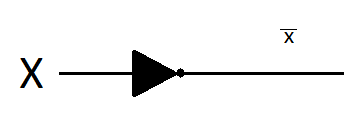
\includegraphics[width=6cm]{img/circuito1.png}
    \end{center}
{\bf b)$\overline{(\overline{x}+z)(y+\overline{z})} \equiv \overline{(\overline{x}+z)}+\overline{(y+\overline{z})} \equiv (\overline{\overline{x}}\overline{z})+(\overline{y}\overline{\overline{z}})$}
\begin{center}                  
      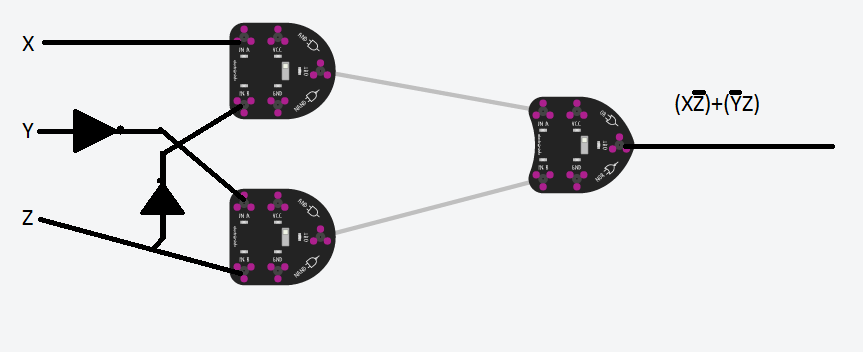
\includegraphics[width=6cm]{img/circuito2.png}
    \end{center}
{\bf c) El circuito recibe dos números compuestos por dos bits x= (x1,x2), y=(y1,y2). La salida del circuito es 1 cuando x>y, 0 en cualquier otro caso}\\
$\overline{x1}x2\overline{y1y2}+x1\overline{x2y1}y2+x1x2\overline{y1y2}+x1x2\overline{y1}y2+x1x2y1\overline{y2}$\\
Usando Mapas-k:
\begin{tabular}{|c|c|c|c|c|}\hline 
   & y1y2 & $y1\overline{y2}$ & $\overline{y1y2}$ & $\overline{y1}y2$ \\ \hline
 x1x2  &  & 1 & 1 & 1 \\ \hline
 $x1\overline{x2}$ & &  & 1 & 1\\ \hline
 $\overline{x1x2}$ & & & & \\ \hline
 $\overline{x1}x2$ & & & 1 & \\ \hline 
\end{tabular}\\
La funcion nos queda reducida $x1\overline{y1}+x1x2\overline{y2}+x2\overline{y1y2}$\\
\begin{center}                  
      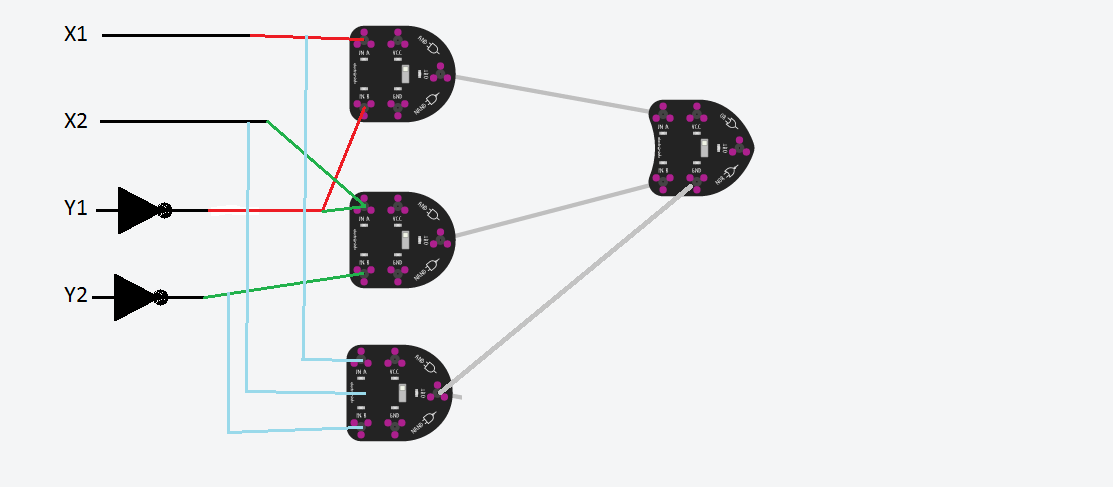
\includegraphics[width=10cm]{img/circuito3.png}
    \end{center}
 {\Large{\bf 3.-Para los siguientes circuitos, encuentra la función booleana que los representa:}}\\
 \begin{center}                  
      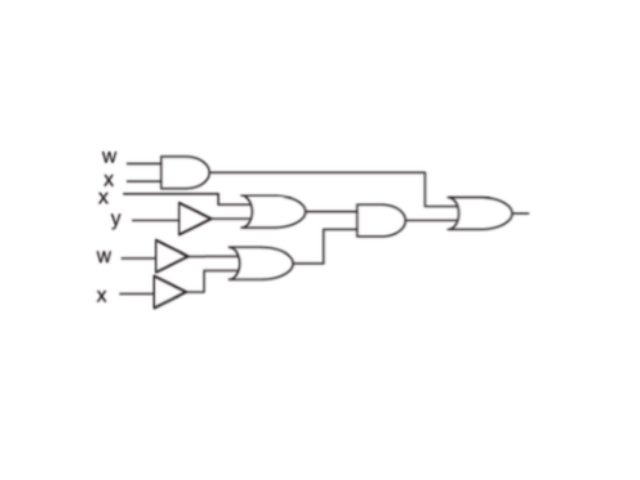
\includegraphics[width=10cm]{img/circuit1.png}
    \end{center}
 El circuito representa la funcion : $(wx)+((x+\overline{y})(\overline{w}+\overline{x}))$\\
 \newpage
 \begin{center}                  
      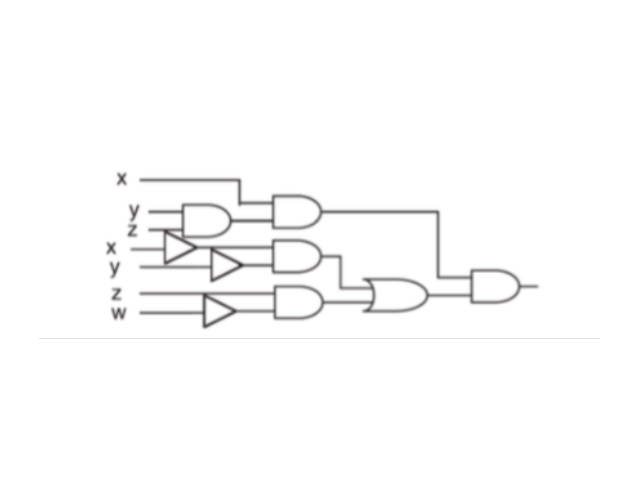
\includegraphics[width=10cm]{img/circuit2.png}
    \end{center}
     El circuito representa la funcion : $(xyz)(\overline{xy}+z\overline{w})$\\

 \newpage
{\Large{\bf 4.-Para cada una de las siguientes fórmulas, decide cuáles son expresiones bien formadas de la lófica de primer orden, justifica. Además, en el caso de estar bien formadas, indica el alcance de cada cuantificador y para cada presencia de variable si es libre o ligada}}\\
{\bf a) $\forall x (\exists yP(x,g(a))) \rightarrow \exists zQ(x,z)$}\\
\begin{forest}
[E
	[E
		[$\forall$]
		[var
			[x
				[deligada]
			]
		]
		[E
			[(]
			[E
				[$\exists$]
				[var
					[y
						[deligada]
					]
				]
				[E
					[Pred
						[P]
					]
					[(List-term)
						[term
							[var
								[x
									[ligada]
								]
							]
						]
						[(list-term)
							[term
								[funcion
									[g]
									[(constante)
										[a]
									]
								]
							]
						]
					]
				]
			]
			[)]
		]
	]
	[$\rightarrow$]
	[E
	[$\exists$]
	[var
		[z
			[deligada]
		]
	]
	[E
		[Pred
			[Q]
		]
		[(list-term)
			[term
				[var
					[x
						[libre]
					]
				]
			]
			[list-term
				[term
					[var
						[z
							[ligada]
						]
					]
				]
			]
		]
	]
	]
]
\end{forest}\\
Utilizando la gramatica de predicados pudimos demostrar que si se puede obtener la cuantificacion a), y en el mismo mostramos cuales son las variables ligadas y cuales las libres.\\
alcance de cuantificador:\\
$\forall x(\exists yP(x,g(a)))$\\
$\exists yP(x,g(a))$\\
$\exists zQ(x,z)$\\

{\bf b)$\neg \forall x\forall yP(x,y,z)\rightarrow g(x,y)$}\\
El inciso b) es incorecto ya que hay una funcion $g(x,y)$ que no esta dentro de un predicado, y la funcion es un termino, y no hay una regla gramatical que permita que $E::= term$, por lo tanto, la sintaxis es incorrecta.\\

{\bf c) $\exists x\exists yQ(x,y) \wedge P(y,z)\rightarrow \forall z\forall yQ(b,z)$}\\
\begin{forest}
[E
	[E
		[E
			[$\exists$]
			[var
				[x
					[deligado]
				]
			]
			[E
				[$\exists$]
				[var
					[y
						[deligado]
					]
				]
				[E
					[Pred
						[Q]
					]
					[(List-term)
						[term
							[var
								[x
									[ligada]
								]
							]
						]
						[list-term
							[term
								[var
									[y
										[ligada]
									]
								]
							]
						]
					]
				]
			]
		]
		[$\wedge$]
		[E
			[Pred
				[P]
			]
			[(list-term)
				[term
					[var
						[y
							[libre]
						]
					]
				]
				[list-term
					[term
						[var
							[z
								[libre]
							]
						]
					]
				]
			]
		]
	]
	[$\rightarrow$]
	[E
		[$\forall$]
		[var
			[z
				[deligado]
			]
		]
		[E
			[$\forall$]
			[var
				[y
					[deligado]
				]
			]
			[E
				[Pred
					[Q]
				]
				[(list-term)
					[term
						[constante
							[b]
						]
					]
					[list-tem
						[term
							[var
								[z
									[ligada]
								]
							]
						]
					]
				]
			]
		]
	]
]
\end{forest}\\
Como podemos ver, la expresion del inciso c)es representable a trávez de las reglas gramaticales, por lo que su sintaxis es correcta.
el alcance de cada cuantificador es:
$\exists x \exists yG(x,y)$\\
$\exists yG(x,y)$\\
$\forall z \forall yQ(b.z)$\\
$\forall yQ(b.z)$\\
{\bf d) $\forall x\forall y(R(x)\rightarrow Q(y,z) \vee \exists f(z)Q(z,y))$}
El inciso d es incorrecto debido aque un cuantificado recibe una variable y un predicado a la derecha de este y en este caso la parte $\exists f(z)Q(z,y))$, podemos ver que el cuantificador recibe una funcion y no una variable, y respecto a las reglas gramaticales de los cuantificadores, esto es incorrecto.\\
\newpage
{\Large{\bf 5.- Sea:\\
Ch(x) = a x le gusta el Chocolate.\\
Ca(x) = a x le gusta el Café.\\
Ce(x) = a x le gusta la Cerveza.\\
Expresa las siguientes oraciones en términos de Ch(x), Ca(x) y Ce(x), cuantificadores y conectivos lógicos. el universo del discurso son tus compañeros (estudiantes) del grupo de Estructuras discretas.}}\\
a) A un estudiante, le gusta el chocolate, el café y la cerveza.\\
$\exists x(Ch(x) \wedge Ca(x) \wedge Ce(x))$\\ \\
b) A todos los estudiantes del grupo les gusta el chocolate o el café o la cerveza.\\
$\forall x(Ch(x)\vee Ca(x)\vee Ce(x))$\\ \\
c)Algunos estudiantes les gusta el café y la cerveza pero no el chocolate\\
$\exist x(Ca(x)\wedge Ce(x)\wedge \neg Ch(x))$\\ \\
d)Si a alguien no le gusta la cerveza, entonces a todos los estudiantes les gusta el chocolate o les gusta el café.\\
$\exists x(\neg Ce(x))\rightarrow \forall y(Ch(y)\vee Ca(y))$\\ \\
{\Large{\bf 6.- traduce los siguientes enunciados a lógica de primer orden(indicando el significado de los predicados y constantes utilizados). Niega la fórmula obtenida y utilizando equivalencias, obtén una expresión cuyas negaciones se encuentren únicamente a la izquierda de predicados. Traduce esta expresion resultante al español. Indica el universo del discurso para cada inciso.}}\\ \\
a) Todos los perros tienen pulgas, muerden y aprenden algunos trugos.\\
x = perro\\
P(x)= x tiene pulgas\\
M(x)= x muerde\\
A(x,y)x aprende y\\
T(x)= x es trucos\\
Universo discurso: todos los perros de la calle. \\
$\forall x\exists y(Q(x)\wedge T(y)\rightarrow P(x)\wedge M(x) \wedge A(x,y))$\\

Negandola tenemos:\\
$\neg (\forall x\exists y(Q(x)\wedge T(y)\rightarrow P(x)\wedge M(x) \wedge A(x,y))) $\\
$\exists x \forall y\neg(Q(x)\wedge T(y)\rightarrow P(x)\wedge M(x) \wedge A(x,y))$\\
Por eliminacion de operadores
$\exists x \forall y\neg(\neg(Q(x)\wedge T(y))\vee P(x)\wedge M(x) \wedge A(x,y))$\\
$\exists x \forall y(\neg\neg(Q(x)\wedge T(y))\wedge \neg(P(x)\wedge M(x) \wedge A(x,y)))$\\
$\exists x \forall y((Q(x)\wedge T(y))\wedge \neg(P(x)\wedge M(x)) \vee \neg A(x,y))$\\
$\exists x \forall y((Q(x)\wedge T(y))\wedge (\neg P(x)\vee \neg M(x) \vee \neg A(x,y))$\\

Traduciendo la negacion al españos tenemos: Algun perro, o tienen pulgas o no muerden o no aprenden nigun truco.\\

b)Todos los joalas saben trepar cualquier árbol\\
K(x)= x es koala\\
T(x.y) = x trepa a y\\
A(x)= x es arbol\\
universo discurso: todos los koalas y arboles.\\
$\forall x\forall y(K(x)\wedge A(y)\rightarrow T(x,y))$\\

Negamos la formula:\\
$\exists x \exists y\neg(K(x)\wedge A(y)\rightarrow T(x,y))$\\
$\exists x \exists y\neg(\neg(K(x)\wedge A(y))\vee T(x,y))$\\
$\exists x \exists y(\neg\neg(K(x)\wedge A(y))\wedge \neg T(x,y))$\\
$\exists x \exists y(K(x)\wedge A(y)\wedge \neg T(x,y))$\\

Traduciendo la negación a español: algunos koala no puede trepar algunos arbol.\\

c)Ningun mono sabe hablar Francés y ningun conejo sabe álgebra\\
M(x) = x es mono\\
F(x) = x puede hablar frances\\
C(x) = x es conejo\\
A(x) = x sabe algebra\\
universo discurso: todos los animales.\\
$\forall x(M(x)\rightarrow \neg F(x)) \wedge \forall y(C(y)\rightarrow \neg A(y))$\\

Negamos la formula\\
$\neg(\forall x(M(x)\rightarrow \neg F(x)) \wedge \forall y(C(y)\rightarrow \neg A(y)))$\\
$\exists x\neg(M(x)\rightarrow \neg F(x)) \vee \exists y\neg(C(y)\rightarrow \neg A(y))$\\
$\exists x\neg(\neg M(x)\vee \neg F(x)) \vee \exists y\neg(\neg C(y)\vee \neg A(y))$\\
$\exists x(\neg\neg M(x)\wedge \neg\neg F(x)) \vee \exists y(\neg\neg C(y)\wedge \neg\neg A(y))$\\
$\exists x( M(x)\wedge F(x)) \vee \exists y( C(y)\wedge A(y))$\\

Traducimos la formula a español: algunos monos saben Francés o algunos conejos saben álgebra\\

d) Exite un cerdo que puede nadar y atrapar algunas mariposas.
C(x) = x es un cerdo.\\
N(x) = x sabe nadar.\\
A(x,y) = x atraba a y\\
M(x) = x es una mariposa.\\
Universo discuros: todos los cerdos del mundo.
$\exists x \exists y(C(x) \wedge M(y) \wedge N(x) \wedge A(x,y))$\\

Negamos la formula\\
$\neg(\exists x \exists y(C(x) \wedge M(y) \wedge N(x) \wedge A(x,y)))$\\
$\equiv\forall x \forall y\neg(C(x) \wedge M(y) \wedge N(x) \wedge A(x,y))$\\
$\equiv\forall x \forall y(\neg(C(x) \wedge M(y)) \vee \neg(N(x) \wedge A(x,y)))$\\
$\equiv\forall x \forall y(\neg C(x) \vee \neg M(y)) \vee (\neg N(x) \vee \neg A(x,y)))$\\
$\equiv\forall x \forall y(\neg C(x) \vee \neg M(y) \vee \neg N(x) \vee \neg A(x,y))$\\

Traducimos al español: Ningun cerdo o no nada o no atrapa ninguna mariposa.\\ \\
e)si todas las aves pueden volar, entonces no hay una jirafa que pueda hablar.\\
A(x)= x es ave.\\
V(x)= x puede volar\\
J(x)= x es jirafa.\\
H(x)= x puede hablar.\\
Universo discuros. Todas las jirafas y aves del mundo.\\
$\forall x(A(x)\wedge V(x)) \rightarrow \neg\exists y(J(y)\wedge H(y))$\\

Negamos la formula:\\
$\neg(\forall x(A(x)\wedge V(x)) \rightarrow \neg\exists y(J(y)\wedge H(y)))$\\
Eliminamos la implicacion
$\equiv \neg(\neg(\forall x(A(x)\wedge V(x))) \vee \neg\exists y(J(y)\wedge H(y)))$\\
$\equiv \neg(\neg(\forall x(A(x)\wedge V(x))) \vee \neg\exists y(J(y)\wedge H(y)))$\\
$\equiv\neg\neg\forall x(A(x)\wedge V(x)) \wedge \neg\neg\exists y(J(y)\wedge H(y))$\\
$\equiv\forall x(A(x)\wedge V(x)) \wedge \exists y(J(y)\wedge H(y))$\\

Traduccion a español: todas las aves vuelan y existe alguna jirafa que puede hablar.\\

\end{document}
